\chapter{Estado del Arte}
\label{cap:EstadoArte}

\setlength{\parindent}{0pt}

En este capítulo se explicará que es blockchain, como funciona, que tipos hay, así como ver su uso en el presente y que aplicaciones se están desarrollando alrededor de la misma para sacarle su máximo potencial, este apartado es de crucial importancia pues servirá para ver el estado del arte de las aplicaciones (en concreto aplicaciones móvil) del presente.

% -------------------------------------------------- %
% -------------------------------------------------- %
\section{Blockchain}
Blockchain\cite{b1,b2,b3} es un término escuchado hoy en día por todas partes, más a nivel económico que tecnológico. Y aunque pueda parecer complejo, su funcionamiento es bastante sencillo.

% -------------------------------------------------- %
\subsection{Definición}
Blockchain es un tipo de base de datos, una base de datos es una colección de información guardada en un ordenador o servidor. Por norma general, la información esta guardada de forma ordenada y estructurada para poder ser accedida con comodidad. Las bases de datos no tienen un tamaño fijo, pudiendo crecer a niveles inimaginables, por norma general solo personal autorizado puede acceder a la información que se encuentra en ellas, así como añadir, eliminar y modificarla. \\

Entonces, ¿donde difiere la blockchain con una base de datos tradicional? \\

Una de las principales diferencias esta en el modo en el que se guarda la información, blockchain junta la información en grupos conocidos como \textbf{bloques}. Estos bloques tienen capacidad para una cantidad de información, y una vez llenos se enlazan con el bloque anterior con la ayuda de un \textbf{hash}. Un \textbf{hash}\cite{whatIsHash} es un algoritmo que mezcla la información que se le introduce para generar una salida única e irreversible de siempre la misma longitud. \\

\begin{figure}[h!]
  \centering
  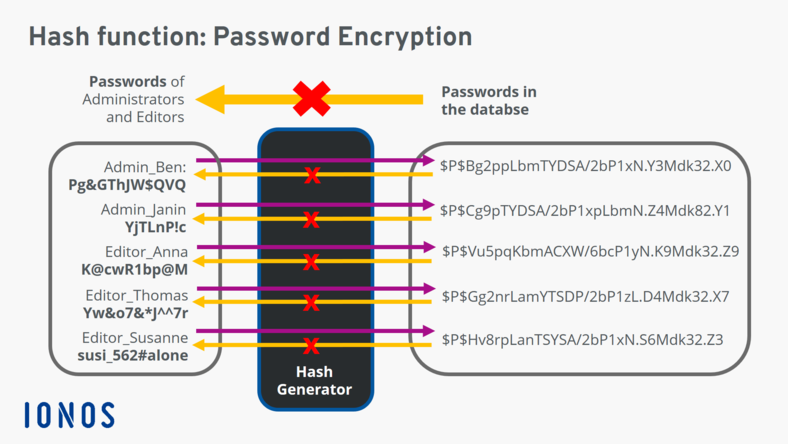
\includegraphics[width=0.6\linewidth]{figs/EstadoArte/Blockchain/hash}
  \caption[Hash]{Ejemplo genérico del funcionamiendo de un algorítmo hash}
  \label{fig:hash}
\end{figure}

\clearpage

Existen múltiples algorítmos hash, y van evolucionando con el tiempo siendo cada vez más seguros y con menos colisiones. Una colisión, se da cuando dos entradas diferentes producen el mismo resultado (rompiendo con una de las reglas principales de los algorítmos hash). \\

Para continuar con la explicación, utilizaremos como ejemplo la red de \textbf{Bitcoin}\cite{whatIsBitcoin} y su algorítmo de consenso \textbf{Proof of Work}\cite{whatIsProofOfWork}. La base es la misma para la inmensa mayoría de redes, sin embargo según el algorítmo de consenso el método difiere ligeramente. Los algorítmos se verán mas adelante. 

\begin{figure}[h!]
  \centering
  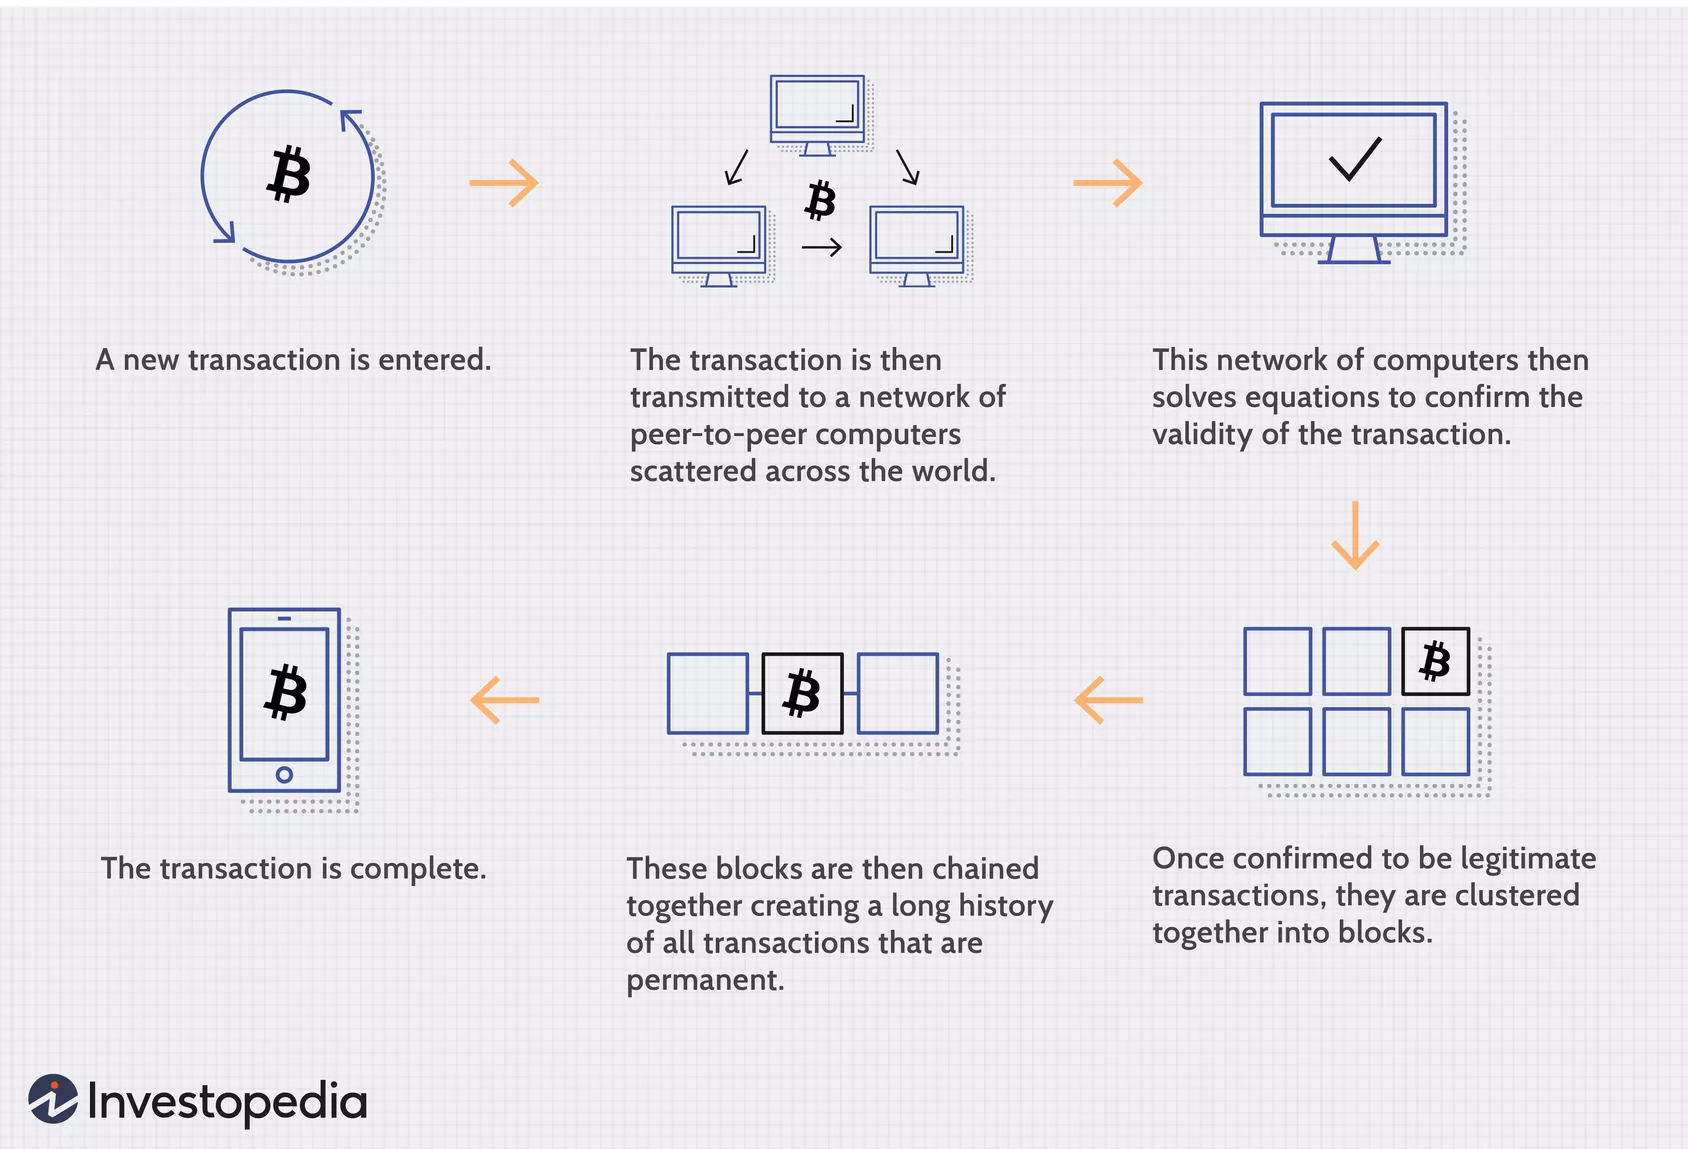
\includegraphics[width=0.8\linewidth]{figs/EstadoArte/Blockchain/bitcoinMining}
  \caption[Bitcoin Mining]{Transaction Process}
  \label{fig:bitcoin}
\end{figure}

Cada bloque de la blockchain, una vez tiene la cantidad de información necesaria para formar un bloque, pasa por una función \textbf{hash256}. Esta información es conocida como ``transacciones'', no son más que datos, ya sean monetarios, envio de datos (nombres, lugares, compras, firmas...) o cualquier tipo de información digital. Todos los nodos de la red comparten estas transacciones, estan todos sincronizados. Él hash por el que pasa la información tiene una especialidad, pues para evitar colisiones entre múltiples nodos de la blockchain, entendemos como nodo un ordenador de la red blockchain, y así evitar que varios bloques se quieran añadir simultaneamente, el hash resultante ha de tener una cantidad determinada de \verb|0|'s al principio del mismo. Por ejemplo, si la dificultad del hash es de \verb|32bits| la función hash256 resultante se puede ver así: \verb|000000003d3a75526946a3bcf00daec9fc9c9c4d51ddc7cc5df888f74dd434d1|. Para llegar a este hash, los nodos de la blockchain tienen que utilizar el hash del bloque anterior junto con la información de las transacciones, y junto con un número conocido como \textbf{nonce}\cite{whatIsNonce}. Un \textbf{nonce} es un número que solo puede ser usado una vez. Los nodos solo pueden modificar este número, no pueden tocar ni el hash del bloque anterior ni las transacciones. Los nodos proceden entonces a modificar de manera aleatoria este nonce hasta dar con el hash con los \verb|0|'s que se piden. Este procedimiento es completamente aleatorio, por lo que a más poder de computo, mas rápido puedes probar números y mas posibilidades tienes de dar con el hash que se pide. A este proceso se le llama ``minado''\cite{minarBitcoin}

\begin{figure}[h!]
  \centering
  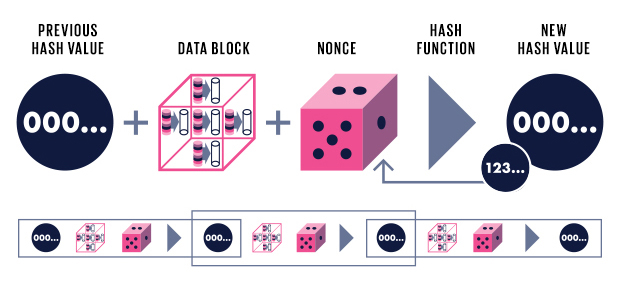
\includegraphics[width=0.8\linewidth]{figs/EstadoArte/Blockchain/hashDificultad}
  \caption[Hash dificultad]{Dificultad del hash}
  \label{fig:hashDiff}
\end{figure}

Una vez un nodo encuentra el nonce correto, lo comparte con el resto de nodos de la red blockchain los cuales validan la información, y se procede a añadir el nuevo bloque a la red blockchain. El nodo que ha encontrado el resultado correcto recibe un incentivo, en el caso de bitcoin, el nodo se asigna a si mismo un número de bitcoins, creando así nuevo bitcoin. 

% -------------------------------------------------- %
\subsection{Tipos de redes blockchain}

Cuando se habla de blockchain, parece dar la impresión de que solo existe un tipo. Sin embargo hay varias redes con sus ventajas y desventajas\cite{tiposBlock1}\cite{tiposBlock2}. Las principales diferencias entre ellas son las \textbf{funcionalidades, protocolos de consenso, administración y reglas para validar las transacciones}.

\subsubsection{Blockchain pública}

Las blockchain públicas no tienen permisos, cualquier usuario es bienvenido a unirse a la red, a enviar transacciones, a utilizar las funcionalidades que tiene la red, y a minar bloques. Las principales características de esta red son:
\begin{itemize}
\item Son \textbf{transparentes}: El código, el funcionamiento interno, los smart contracts si tiene (se verá este término mas adelante) son todos públicos y de código abierto.
\item \textbf{Sin permisos}: Cualquier persona puede unirse a la red sin preguntar. Lo único que tiene que hacer es descargar la red y sincronizarse con los demas nodos.
\item Usuarios \textbf{anónimos} y \textbf{sin administriador}: Nadie se conoce en la red, se trabaja siempre con lo que se conoce como \textbf{address}, que viene a ser un identificador único por miembro de la red para identificarlo. Además, no existe administrador de la red, no hay una persona o grupo que tenga poder sobre la red para hacer cambios de ningún tipo.
\item La información de la red puede ser \textbf{mantenida por todas las personas que lo deseen}. Y al minar nuevos bloques, dependiendo de la red, se ofrece un \textbf{incentivo}.
\end{itemize}

En resumidas cuentas, una blockchain pública es \emph{descentralizada}, \emph{distribuida}, \emph{consensuada}, \emph{abierta} y \emph{segura}. Algunos ejemplos de redes públicas son bitcoin\cite{webBitcoin} y ethereum\cite{webEthereum}

\subsubsection{Blockchain privada}

Las blockchains privadas son permisionadas, esto quiere decir que no cualquier persona puede añadirse como nodo libremente. Requieren de una \textbf{entidad} que ejerza de \textbf{administrador}. La mayoría de usuarios no consideran estas redes como blockchain a causa de esto. El administrador de la red tiene que dar permiso a los usuarios para poder minar, enviar transacciones y participar en general en la red. \\

Admeás, es abitual que los datos esten almacenados en servidores centrales y no abiertos al público. Pudiendo acceder a los bloques de la red solo mediante invitación. \\

Algunos ejemplos de blockchains privadas son R3\cite{webR3}, Ripple\cite{webRipple} y Quorum\cite{webQuorum}

\subsubsection{Blockchain híbrida o federada}

Estas redes son utilizadas por grandes empresas y gobiernos, no estan abiertas al público, teniendo la gestión varias entidades. Además no tienen una criptomoneda asociada y no recompensan por el minado de bloques. Sin embargo el software que utilizan es de código abierto, como puede ser \textbf{Hyperldger, Corda}\cite{webHyper, webCorda}. \\

Como ejemplo tenemos la \emph{Enterprise Ethereum Alliance}, en la que participan el Banco Santander y BBVA. Esta red utiliza la blockchain de Ethereum (pública), sin embargo tienen su propia plataforma privada.

\subsubsection{Blockchain as a Service}

Estas redes blockchain son controladas por un proveedor de servicios como puede ser \emph{Amazon}. Estos proveedores permiten utilizar redes blockchain en la nube, permitiendo a los desarrolladores aprovechar el potencial de las redes blockchain sin la necesidad de invertir en el computo que ello requiere.

% -------------------------------------------------- %
\subsection{Tipos de algoritmo de consenso}

\begin{figure}[h!]
  \centering
  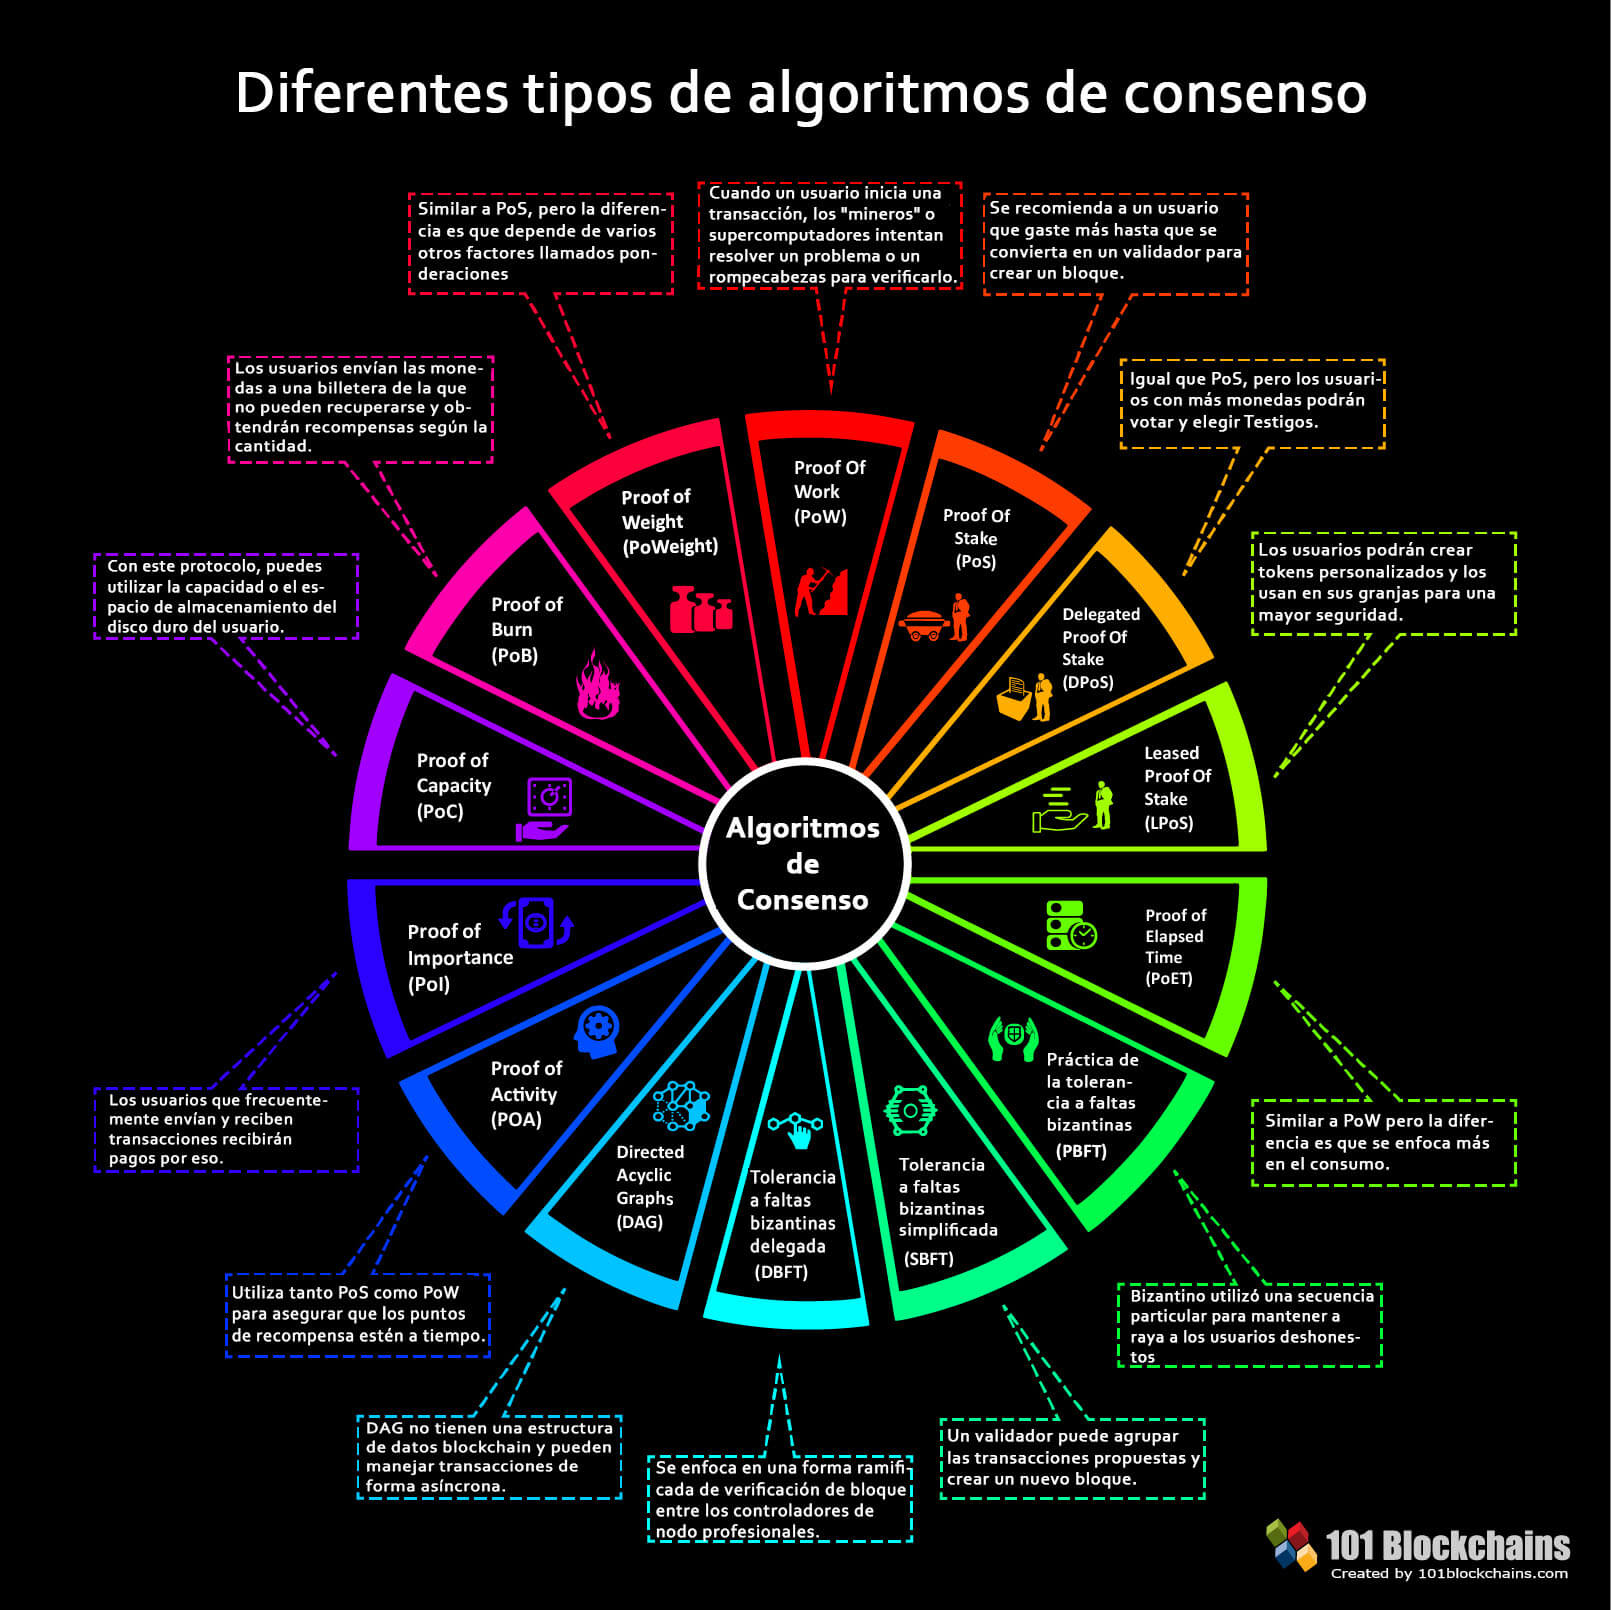
\includegraphics[width=0.8\linewidth]{figs/EstadoArte/Blockchain/algoritmosConsenso.jpeg}
  \caption[Algoritmos de Consenso]{Diferentes tipos de algoritmos}
  \label{fig:consenso}
\end{figure}

Existen múltiples algoritmos de consenso, y estos evolucionan con el paso del tiempo. Los algoritmos de consenso son procesos o protocolos de toma de decisiones, dependiendo del algoritmo hay uno o varios nodos de la red con el poder de tomar la decision sobre que bloque es el siguiente en añadirse a la red y si ha sido o no alterado. Los objetivos que busca blockchain con los algoritmos de consenso son:

\begin{itemize}
\item Llegar a un acuerdo
\item Cooperación
\item Colaboración
\item Igualdad de derechos
\item Participación
\item Actividad
\end{itemize}

Puesto que hay una gran cantidad de algoritmos trataremos de explicar algunos a continuación\cite{algoConsenso}. Todos los algoritmos buscan el mismo objetivo, solucionar el problema de las \textbf{faltas bizantinas}(BFT)\cite{BFT}. La tolerancia a faltas bizantinas es la resistencia de un sistema informático tolerante a fallas de componentes electrónicos. Si lo llevamos al mundo blockchain, cuando hablamos de fallas nos referimos a nodos de la blockchain defectuosos accidentalmente o provocado. Si una empresa tiene control de 200 nodos, puede tratar de crear transacciones falsas y minar ese bloque con los 200 nodos, el resto de nodos de la red tienen que ser capaces a través del algoritmo de consenso que se utilice de descartar la información de estos 200 nodos.

\subsubsection{Proof of Work (PoW)}

El algoritmo de prueba de trabajo es el primer algoritmo introducido en la red blockchain. Muchas blockchains utilizan este algoritmo para llevar a cabo el consenso y así confirmar todas las transacciones. \\ 

\emph{¿Como funciona?} Cada nodo tiene descargada la red blockchain entera, cuando el nuevo bloque tiene las transacciones necesarias para ser minado, todos los nodos se ponene a buscar el resultado de un \textbf{hash} con la dificultad que tenga el mismo. A más poder de computo, mas posibilidades de encontrar el resultado, validarlo con los otros nodos y añadirlo a la red blockchain, además las redes que usan PoW suelen tener un sistema de premios por lo que cuando un nodo encuentra la solución al problema se le da criptomonedas a cambio. \\

Este sistema tiene dos principales desventajas, la primera es que el poder de cálculo que se necesita es muy grande, y estos últimos años han crecido lo que se conoce como granjas de minado las cuales se llevan el premio la gran mayoría de veces. Esto causa que el sistema empiece a centralizarse, rompiendo con la idea de descentralización que tiene blockchain. El problema es que si alguien logra tener él poder de computo de un 51\% de la red blockchain este puede añadir los bloques que quiera a partir de ese momento pues siempre serán validados por la mayoría de nodos (su 51\% de los nodos). La segunda gran pega va liagada a estas granjas de minado, consumen gran cantidad de energía, en 2020 bitcoin consumió \emph{120 gigawatts} por segundo\cite{bitcoinEnergyUse} lo que a nivel medioambiental tiene un impacto negativo, por lo que PoW no es un algoritmo de consenso que se pueda mantener en el tiempo.

\emph{Ventajas y Desventajas}
\begin{itemize}
\item PROS
  \begin{itemize}
  \item Evita ataques DDoS
  \item Es justo y transparente
  \item Fomenta el interés del público en mantener una red saludable
  \end{itemize}
\item CONS
  \begin{itemize}
  \item La adquisición de equipo para el minado es costosa
  \item La máquina destinada al minado no podrá utilizarse para otra tarea pues se necesita todo el poder de computo en la resolución de los problemas matemáticos.
  \item La red tiende a centralizarse a causa de las granjas de minado, dandole poder al dueño de la granja y rompiendo la descentralización.
  \item La minería desaparecerá cuando no haya mas incentivos, en el caso de Bitcoin, cuando se alcance el límite de Bitcoins (21 Millones) los mineros dejarán de recibir premios y se perderá la motivación del minado.
  \end{itemize}
\end{itemize}

\subsubsection{Proof of Stake (PoS)}

El concepto de participación establece que una persona puede minar o validar transacciones en bloque según el número de monedas que posea. Esto significa que cuanta más criptomoneda tengas, más poder de minado se te asigna. \\ 

Se creó como alternativa a PoW, para solventar algunos problemas que tiene (como el de la centralización a causa de las granjas de minado y el gasto energético derivado del poder de computo). PoS solventa este problema atribuyendo la potencia minera a la proporción de monedas que posee un minero. Por lo tanto, en vez de utilizar energía para responder al puzzle matemático como hace PoW, aquí el minero se limita a resolver un porcentaje de las transacciones. Si se tiene un 3\% de las criptomonedas disponibles, se puede minar un 3\% de los bloques, en esta ocasión no hay que resolver ningun puzzle matemático, simplemente generar un \textbf{hash} con los datos, lo que es una tarea trivial. \\

PoS no es una solución definitiva, pues tiene problemas al igual que PoW. Al igual que antes mencionamos el ataque del 51\% (cuando una empresa o alguien tiene un 51\% de los nodos en su poder). En PoS, si tienes un 51\% de las criptomonedas, tienes un 51\% del poder de decision sobre la red, pudiendo hacer los cambios que quieras en ella. Este ataque es frecuente en redes pequeñas con pocas criptomonedas en juego, puesto que de lo contrario, lograr tener un 51\% de las monedas supone tener muchísimo dinero. Para controlar estas fraudulencias, se penaliza económicamente a los nodos que tratan de saltarse las reglas (modificar bloques y transacciones), además, un ataque a la blockchain afecta al poder de la moneda y por lo tanto su valor en mercado disminuye, por lo que no compensa tratar de burlar las reglas de la blockchain. Los nodos de las redes que usan PoS, reciben una comisión al minar correctamente su parte del bloque. \\

Redes que utilizan este algoritmo son: Ethereum2.0\cite{Ethereum2.0} y NxT\cite{NxT}.

\subsubsection{Proof of Elapsed Time (PoET)}

La prueba de tiempo transcurrido es un algoritmo que evita la alta utilización de recursos y el alto consumo de energía manteniendo el proceso más eficiente. El algorítmo utiliza un tiempo transcurrido generado aleatóriamente para decidir los derechos de minería y los ganadores de los bloques. Al ejecutar un código de confianza dentro de un entorno seguro, el algoritmo PoET también mejora la transparencia al garantizar que los resultados sean verificables por participantes externos. Este algorítmo se utiliza en redes blockchain permisionadas, por lo que se conoce al dueño de cada nodo. \\

Cada nodo participante en la red debe esperar durante un periodo de tiempo elegido al azar, y el primero en completar el tiempo de espera designado gana el nuevo bloque. Cada nodo de la red blockchain genera un tiempo de espera aleatorio y se pone a dormir durante esa duración especificada. El que se despierta primero, es decir, el que tiene el tiempo de espera más corto, se despierta y consigna un nuevo bloque en la cadena de bloques, transmitiendo la información necesaria a toda la red de pares. El mismo proceso se repite para descubrir el siguiente bloque. \\

% -------------------------------------------------- %
\subsection{Smart contracts}

Hasta ahora, hemos hablado de blockchain y criptomonedas, pero las criptomonedas son solo un muy pequeño uso del potencial de blockchain. Los \textbf{Smart Contracts}\cite{etherSmartContract} son un programa que se ejecuta en la red blockchain dando así la capacidad a la red de ser más versatil, al poder ejecutar código (escrito en el smart contract). Básicamente, añade una lógica a la blockchain. \\

Una forma de entender los smart contracts es comparandolos a una máquina de ventas automática. Cuando quieres un snack introduces dinero en la máquina y pones el código del snack, la máquina tiene programada una rutina para verificar que has metido la cantidad adecuada y a cambio devuelve el snack seleccionado. Ese programa interno que tiene la máquina, es el equivalente a un \textbf{smart contract}. \\

Los smart contract son muy poderosos al estar programados en la red blockchain no pueden ser modificados sin que todos los nodos se enteren. Si un nodo trata de modificar el smart contract, se creará una transacción la cual ha de ser validada por todos los nodos, al igual que cuando hablabamos de cambiar transacciones en criptomonedas, los algoritmos de consenso se encargarán de prohibir que nodos no permitidos cambien componentes del smart contract. \\

Los smart contracts permiten que se realicen transacciones y acuerdos de confianza entre partes dispares y anónimas sin necesidad de una autoridad central, un sistema legal o un mecanismo de aplicación externo. \\

\label{sec:smartContract}
\index{SmartContract}

\begin{lstlisting}[language=Java,float=ht,caption={[Smart Contract]Ejemplo de código fuente de un smart contract escrito en Solidity},label=lst:java]
pragma solidity 0.6.11;

contract VendingMachine {

    // Declare state variables of the contract
    address public owner;
    mapping (address => uint) public cupcakeBalances;

    // When 'VendingMachine' contract is deployed:
    // 1. set the deploying address as the owner of the contract
    // 2. set the deployed smart contract's cupcake balance to 100
    constructor() public {
        owner = msg.sender;
        cupcakeBalances[address(this)] = 100;
    }

    // Allow the owner to increase the smart contract's cupcake balance
    function refill(uint amount) public {
        require(msg.sender == owner, "Only the owner can refill.");
        cupcakeBalances[address(this)] += amount;
    }

    // Allow anyone to purchase cupcakes
    function purchase(uint amount) public payable {
        require(msg.value >= amount * 1 ether, "You must pay at least 1 ETH per cupcake");
        require(cupcakeBalances[address(this)] >= amount, "Not enough cupcakes in stock to complete this purchase");
        cupcakeBalances[address(this)] -= amount;
        cupcakeBalances[msg.sender] += amount;
    }
}
\end{lstlisting}

Los smart contracts pueden ser escritos en múltiples lenguajes de programación dependiendo de la red blockchain que se vaya a utilizar. Algunos ejemplos son:
\begin{itemize}
\item EOS Blockchain -> \verb|C++|
\item Ethereum -> \verb|Solidity|
\item NEO Blockchain -> \verb|JavaScript, Java|
\item Hyperldger -> \verb|Golang|
\item Cardano -> \verb|Haskell|
\end{itemize}

La primera red blockchain en explotar el potencial de los smart contracts fue \textbf{ethereum} y puesto que es la red blockchain sobre la cual se apoyará la aplicación Android que voy a desarrollar en este TFG, procederé a analizarla.

% -------------------------------------------------- %
\subsection{Usos en el presente de Blockchain}
En el presente estan en desarrollo múltiples aplicaciones basadas en Blockchain:

\begin{itemize}
\item Criptomonedas: \emph{Bitcoin, Ethereum, Tether, Cardano, XRP, Litecoin, ChainLink, Dogecoin, TRON, VeChain, Monero, BitTorrent, Kusama, Neo, Dai, NEM, Dash, Maker}\dots \cite{listaCripto}.
\item Firma digital y verificación de la identidad: Startups como \emph{Civic} o \emph{Niuron}\cite{civic, niuron} buscan implementar firmas digitales para notarios y bancos y check-in telemáticos en hoteles y pisos turísticos.
\item Trazabilidad alimentaria: Empresas como carrefour implementan trazabilidad de sus alimentos con la ayuda de IBM \cite{carrefour}
\item Turismo y Hoteles: La empresa \emph{TUI Group} cuenta con más de 300 hoteles y esta moviendo sus activos inmobiliarios y procesos internos a una blockchain \cite{tuig}.
\item Votaciones y elecciones: El \emph{banco santander} utilizó en 2018 con éxito una red blockchain para votar a su Junta General de Accionistas\cite{santanderVotacion}
\end{itemize}

Y mucho más \cite{appCripto}.

% -------------------------------------------------- %
\section{Ethereum}

\begin{figure}[h!]
  \centering
  
\includegraphics[width=0.6\linewidth]{figs/EstadoArte/Ethereum/ethereumLOGO}
  \caption[Ethereum]{Logo de ethereum}
  \label{fig:ethereum}
\end{figure}

Ethereum es una red blockchain que permite enviar criptomonedas a cualquier persona por una pequeña comisión. Admeás permite ser programada con ayuda de los smart contracts, permitiendo así desarrollar aplicaciones sobre la red blockchain. \\

% -------------------------------------------------- %
\subsection{Ether (ETH)}
La moneda que utiliza la red de Ethereum es el \textbf{ether}, se utiliza para compensar a los mineros que aseguran las transacciones. Recordemos, \emph{Ethereum1.0 utiliza PoW} pero \emph{Ethereum2.0 utiliza PoS}\cite{Ethereum2.0}. Los ethers se utilizan como almacén de valor, prestamos de garantía, medio de intercambio, unidad de cuenta en mercados digitales \dots \\

Cada transacción en ethereum lleva asociado un coste conocido como \textbf{gas}. El gas es la unidad que se utiliza para ver el coste de computo que tiene la transacción, para poder remunerar adecuadamente al minero. La unidad de gas se mide en \textbf{Gwei}\cite{Gwei} si por ejemplo queremos enviar una cantidad \verb|X| de ether a otra persona esta transacción tiene un coste de \verb|21.000|Gwei lo que es equivalente a \verb|0,000021 ETH| (1ETH = $10^9$Gwei)

% -------------------------------------------------- %
\subsection{Carteras}

Las carteras de ethereum son aplicaciones que permiten a los ususarios interactuar con sus cuentas de ethereum. Se las puede ver como una aplicación bancaria. Tu cartera te permite leer tu saldo, enviar transacciones y conectarte a aplicaciones. Se necesita una cartera para enviar fondos y gestionar tu ETH. Pero es únicamente una herramienta para gestionar tu cuenta, puedes cambiar de cartera sin problema pues no es quien custodia tus fondos, eres tú quien los custodia en todo momento. \\

La cartera tiene asociado un \textbf{address}, un address es el identificador que tiene tu cuenta en la red de ethereum, es único para tí. Si alguien quiere enviarte dinero lo hará desde su address a tú address, si quieres hacer una llamada a un Smart Contract, al smart contract le llegará como información tú address. \\

Tres términos importantes:
\begin{itemize}
\item \textbf{Cuenta} de ethereum.
\item \textbf{Address} de la cuenta.
\item \textbf{Cartera} para gestionar la cuenta.
\end{itemize}

% -------------------------------------------------- %
\subsection{Ethereum Smart Contract}

Los smart contracts de ethereum están escritos en \textbf{Solidity}\cite{SolidityDocs} o \textbf{Vyper}\cite{VyperDocs}. Cualquier persona es libre de programar un smart contract y desplegarlo en la red de ethereum, los smart contracts son una transacción más y tienen su propio address. Permitiendo que cualquier persona hacer llamadas al smart contract. Desplegar un smart contract cuesta \emph{gas} al igual que cualquier transacción, sin embargo es bastante más caro. 

\begin{figure}[hbt]
	\centering
	\begin{subfigure}[b]{0.4\linewidth}
		\centering
		
\includegraphics[width=0.8\linewidth]{figs/EstadoArte/Ethereum/solidityLOGO}
		\caption{Logo de Solidity}\label{fig:solProgram}
	\end{subfigure} 
	\begin{subfigure}[b]{0.4\linewidth}
		\centering
		
\includegraphics[width=0.8\linewidth]{figs/EstadoArte/Ethereum/vyperLOGO}
		\caption{Logo de Vyper}\label{fig:vyperProgram}
	\end{subfigure} 
	\caption[Lenguajes de Smart Contract]{Lenguajes de smart contract para ethereum.}
	\label{fig:programas}
\end{figure}

\clearpage

\label{sec:solidity}
\index{Solidity}

\begin{lstlisting}[language=Java,float=ht,caption={[Solidity Contract]Ejemplo de código fuente de un smart contract escrito en Solidity},label=lst:java]
// SPDX-License-Identifier: GPL-3.0
pragma solidity >= 0.7.0;

contract Coin {
    // The keyword "public" makes variables
    // accessible from other contracts
    address public minter;
    mapping (address => uint) public balances;

    // Events allow clients to react to specific
    // contract changes you declare
    event Sent(address from, address to, uint amount);

    // Constructor code is only run when the contract
    // is created
    constructor() {
        minter = msg.sender;
    }

    // Sends an amount of newly created coins to an address
    // Can only be called by the contract creator
    function mint(address receiver, uint amount) public {
        require(msg.sender == minter);
        require(amount < 1e60);
        balances[receiver] += amount;
    }

    // Sends an amount of existing coins
    // from any caller to an address
    function send(address receiver, uint amount) public {
        require(amount <= balances[msg.sender], "Insufficient balance.");
        balances[msg.sender] -= amount;
        balances[receiver] += amount;
        emit Sent(msg.sender, receiver, amount);
    }
}
\end{lstlisting}

% -------------------------------------------------- %
\subsection{Funcionamiento básico de Ethereum}

Para entender el funcionamiento básico de Ethereum, vamos a exponerlo por niveles como lo hacen en la documentación oficial\cite{etherStack}. 

% -------------------------------------------------- %
\subsection{Nivel 1: Máquina Virtual de Ethereum} 

La \textbf{EVM} es el entorno de ejecución de los smart contract. Esta, gestiona todo el procesamiento de transacciones en la red, creando un nivel de abstracción entre el código que se ejecuta y la máquina que lo hace. La EVM es \emph{Turing-Completa} con 140 instrucciones únicas que la permiten ejecutar casi cualquier cosa. 

\begin{figure}[h!]
  \centering
  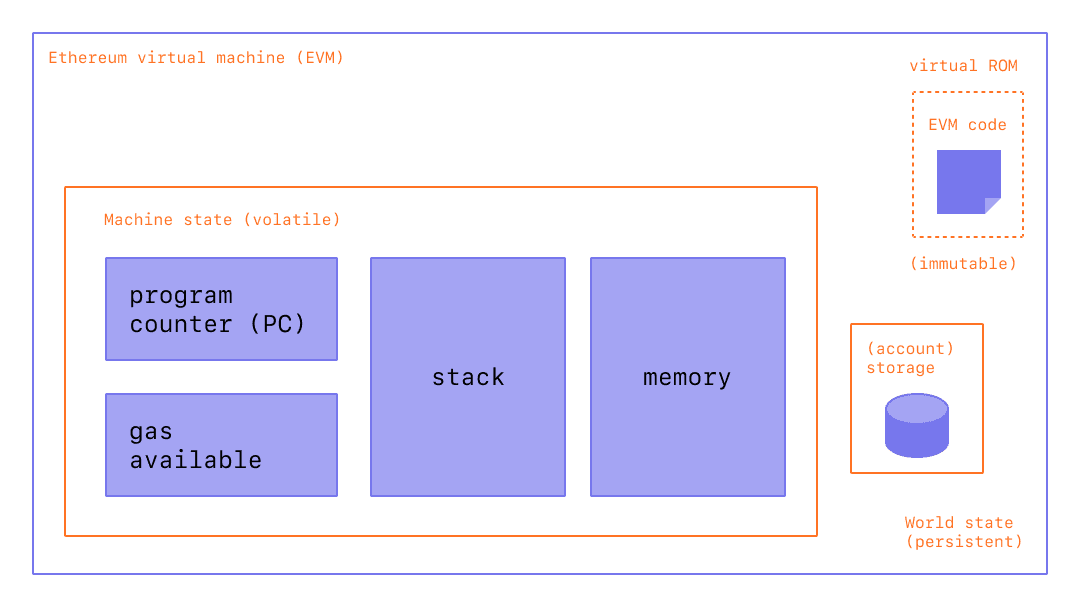
\includegraphics[width=0.6\linewidth]{figs/EstadoArte/Ethereum/evm}
  \caption[Diagrama EVM]{Diagrama de la máquina virtual de ethereum}
  \label{fig:evm}
\end{figure}

% -------------------------------------------------- %
\subsection{Nivel 2: Smart Contract} 

Programas que se ejecutan en la red de ethereum. 

% -------------------------------------------------- %
\subsection{Nivel 3: Nodos de Ethereum}

Para que una app pueda interactuar con la red, necesita conectarse a un nodo de ethereum. Los nodos son ordenadores que ejecutan el \emph{software} cliente de ethereum, manteniendo el registro de bloques y validando las transacciones. Almacenan colectivamente el estado de la blockchain y llegan a un consenso sobre las transacciones para hacer crecer el número de bloques. Al conectar la app con un nodo, la app puede leer datos de la red, enviar nuevas transacciones\dots

\begin{figure}[h!]
  \centering
  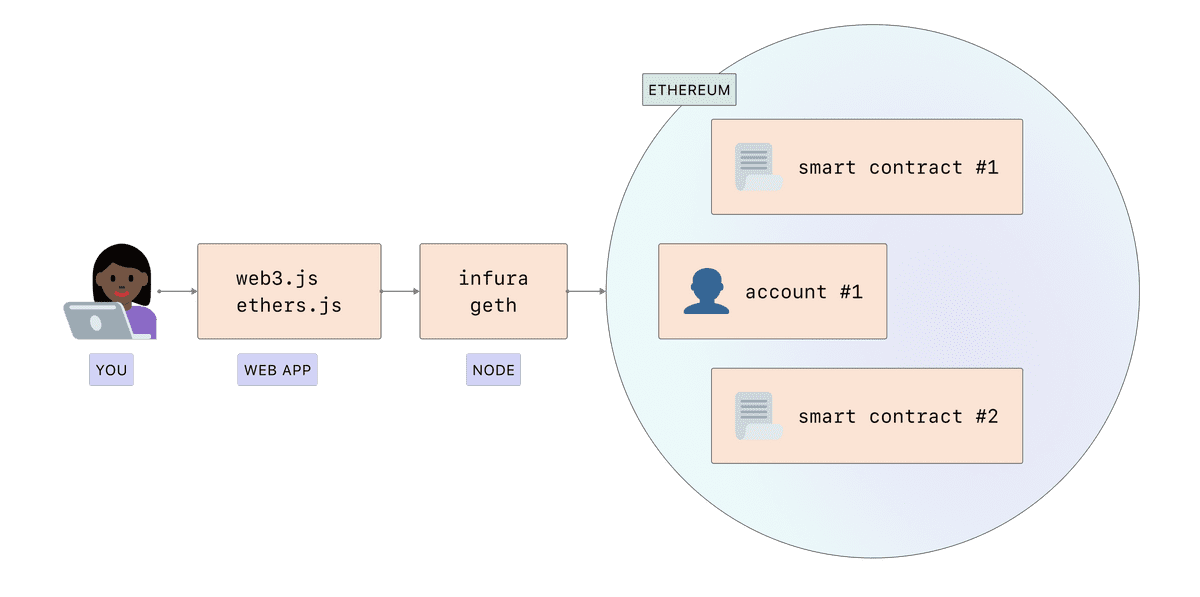
\includegraphics[width=0.6\linewidth]{figs/EstadoArte/Ethereum/ethereumNodo}
  \caption[Nodos vista genérica]{Nodo y vista genérica de aplicaciones.}
  \label{fig:etherNodo}
\end{figure}

% -------------------------------------------------- %
\subsection{Nivel 4: API para el cliente de ethereum}

Las APIs permiten a los desarrolladores absatraer parte de la dificultad de interactuar directamente con los nodos de ethereum. Además proporcionan herramientas como para convertir datos de ETh a Gwei\dots Existen APIs en \verb|JavaScript, Java, Python| por ejemplo, una de las más conocidas es \textbf{Web3}\cite{web3}

% -------------------------------------------------- %
\subsection{Nivel 5: Aplicaciones para usuario}

En el nivel superior estan las apps orientadas al usuario. Principalmente son aplicaciones web y móvil. Las aplicaciones se contruyen de la manera tradicional, y utilizan las APIs necesarias para comunicarse con la red y/o smart contracts.

% -------------------------------------------------- %
% -------------------------------------------------- %
\section{Aplicaciones móvil que usan Blockchain}

Ahora que entendemos que es Blockchain, visto múltiples ejemplos de redes, visto múltiples aplicaciones de la red Blockchain, y hemos indagado más sobre Ethereum y lo Smart Contract, vamos a pasar a ver los proyectos actuales que utilizan aplicaciones móvil y blockchain. Puesto que el objetivo de este \textbf{TFG} es el desarrollo de una aplicación Android que comunique con una blockchain. 

% -------------------------------------------------- %
\subsection{GUTS Tickets}

Esta aplicación móvil usa blockchain para emitir entradas honestas que ponen fin a los vergonzosos precios del mercado de la ``reventa'' y al fraude en las entradas. \emph{GUTS} es el primer sistema de ventas de entradas que hace uso del \textbf{Protocolo de Entrada Garantizada} {\small (\emph{Guaranteed Entrance Protocol (GET)})}\cite{GET}. Este protocolo permite crear entradas inteligentes y seguras permitiendo el seguimiento de las mismas así como el control de su precio original y secundario (reventa). 

\begin{figure}[hbt]
	\centering
	\begin{subfigure}[b]{0.4\linewidth}
		\centering
		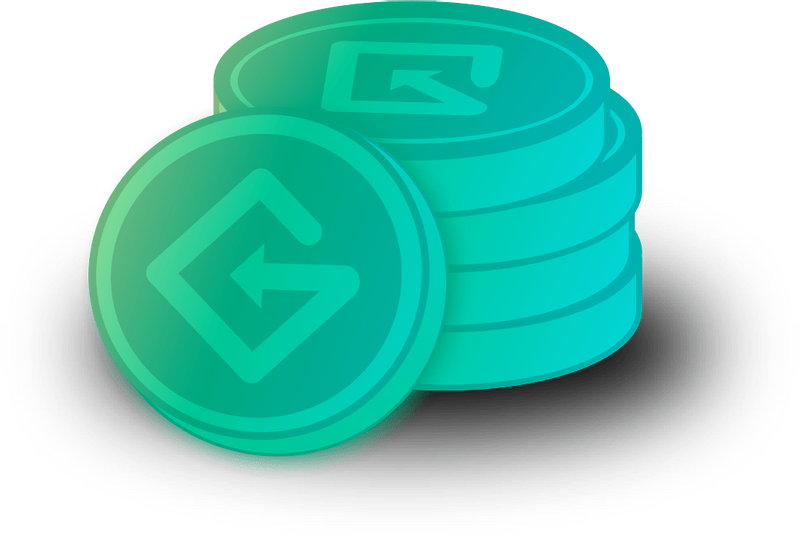
\includegraphics[width=0.8\linewidth]{figs/EstadoArte/Apps/getTOKEN.png}
		\caption{Logo del token de GET}\label{fig:getTOKEN}
	\end{subfigure} 
	\begin{subfigure}[b]{0.4\linewidth}
		\centering
		
\includegraphics[width=0.8\linewidth]{figs/EstadoArte/Apps/gutsLOGO.png}
		\caption{Logo de la aplicación Guts}\label{fig:gutsLOGO}
	\end{subfigure} 
	\caption[Logos de Guts y GET]{Logos}
	\label{fig:Logos}
\end{figure}

\subsubsection{Protocolo GET}

El protocolo GET ofrece una solución de emisión de billetes inteligentes basadas en blockchain que puede ser utilizada por todos los que necesitan emitir billetes de forma transparente, segura y honesta. Evitando fraudes, y vergonzosas subidas del precio de las entradas en el mercado de la reventa. La funcionalidad de registro de entradas de GET funciona con un SmartContract escrito en solidity, su codigo fuente es de código abierto \cite{srcGET}. La blockchain que utiliza para apoyarse es la de \emph{Ethereum}, y disponen de \textbf{Token} propio para realizar las transacciones\cite{tokGET}. GET guarda un historial para cada tickets utilizando \textbf{IPFS}\cite{IPFS} que luego guarda en la red blockchain con el smart contract, \emph{sobre IPFS, pretende superar a HTTP para contruir una web mejor para todos}.

% -------------------------------------------------- %
\subsection{LifeID}

Esta aplicación esta construyendo una plataforma de identidad digital segura y basada en blockchain. Con una sencilla aplicación móvil te ofrece el control sobre la gestión de tú identidad digital. Permite iniciar sesión en cualquier sitio, entrar en cualquier edificio en el que se requiera de autenticación o participar en transacciones basadas en la identidad (como puede ser en un sistema de votación) todo con la tranquilidad, fiabilidad y control que da la blockchain. \\ 

Para ello utiliza la red blockchain de \textbf{ArcBlock}\cite{webArc,alianzaArc}. ArcBlock es una plataforma para desarrollar aplicaciones en blockchains conocidas como \textbf{DApps}\cite{dapps}. 


